\documentclass[a4paper, 10pt]{article}

\usepackage[margin = 1in]{geometry} % for spacing around
\usepackage{graphicx} % for including images in your pdfs
\usepackage{xcolor} % for including colors in your pdf
\usepackage{soul} % for text decoration
\usepackage[utf8]{inputenc} % for encoded text
\usepackage[T1]{fontenc}
\usepackage{setspace} % for setting different line spacings between paragrafs.
\usepackage{enumerate} % for letting us get more detailed enumerate lists
\usepackage{multirow} % to let us combine more rows together
\usepackage{colortbl} % for decorating tables
\usepackage{amsmath} % used for representing more complicated math displays
\usepackage{supertabular}
\usepackage{longtable} % both of these packages are used to making really big tables
\usepackage{wrapfig} % allows us to wrap text around figures
\usepackage{fancyhdr} % for making fancy headers
%\usepackage{bibtex} % for making better bibliographies
\usepackage[pdftex]{hyperref} % for letting us make links
\usepackage{lscape} % Allows us to flip from portrait to landspace
\usepackage{tikz} % for high detailed drawing
\usepackage{multicol} % To put things side by side
\usepackage{rotating} % For rotating objects
% \usepackage{draftwatermark} % For adding watermarks
\usepackage{MnSymbol} % for using multiple symbols
\usepackage{mathtools} % Used for more math symbols
\usepackage{xfrac} % For more complciated fractions and to add derivitives
\usepackage{hyperref} % for hyper links
\usepackage{enumitem} % for better enum lists
\usepackage{tcolorbox} % for adding colored text boxes
\usepackage{bm} % Adding bold text to math inputs
\usepackage{pgfplots} % Used for plotting functions
\usepackage{subcaption} % Used for adding multiple images in one figure

% Setting up the default image path
\graphicspath{{../../global-assets/images/}}

% Implementing authro details
\title{Lab Report number VII - Capacitors\\
	ENS203 - Electrical Circuits I}
\author{Emre Arapcic-Uevak\\220302289}
\date{}

% Setting up the fancy page style
\fancypagestyle{customStyle}{
	\lhead{} \chead{} \rhead{}
	\lfoot{} \cfoot{\thepage} \rfoot{}
	\renewcommand{\headrulewidth}{0pt}
	\renewcommand{\footrulewidth}{1pt}
}
\pagestyle{customStyle}

% Setting up hyperref options
\hypersetup {
	colorlinks = false,
	citecolor = black,
	filecolor = blue,
	linkcolor = blue,
	urlcolor = blue,
	pdftex
}

% Custom commands


\begin{document}
	\begin{titlepage}
		\begin{center}
			\vspace*{\stretch{1}} % Add vertical space before the title

			{\Large\bfseries Lab Report number 7 \\[0.5em] Capacitors\par}
			\vspace{1cm} % Space between title and course title

			{\large ENS203 – Electrical Circuits I\par}
			\vspace{1cm} % Space between course title and your name/ID

			{\large Emre Arapcic-Uevak \\ 220302289\par}
			\vspace{1cm} % Space between your name/ID and assistant name

			{\large Afan Haznadarevic \\ 220302128\par}
			\vspace{.5cm} % Space between your name/ID and assistant name

			{\large Assistant: Adil Hasanbasic\par}
			\vspace{\stretch{2}} % Variable vertical space between assistant name and bottom
			
\includegraphics[width=0.5\textwidth]{Logo.png}
			\vspace{5mm}
			
			\textsc{\LARGE Internation University of Sarajevo}\\[1.5cm]
			\textsc{\Large ENS203 - Electrical Circuits I}\\[0.5cm]
			
			\rule{\linewidth}{0.5mm} \\[0.4cm]
			{ \huge \bfseries Lab Report number VII - Capacitors}\\[0.4cm]
			\rule{\linewidth}{0.5mm} \\[1.5cm]
			
			\vfill
			
			% Bottom of the page
			{\large \today}
		\end{center}
	\end{titlepage}
	\pagebreak

	\tableofcontents
	\pagebreak
	
	\listoffigures
	\pagebreak
	
	\section{Introduction}
		In this lab, we will be analyzing the behavior of capacitors in DC circuits. 
		We will be measuring the voltage across the capacitor and how long it takes to charge the capacitor depending on the resistance and capacitance of the circuit.

		\subsection{Theoretical Background}
			Capacitors are passive electrical components that store energy in the form of an electric field. 
			The capacitance of a capacitor is the ability of the capacitor to store energy.\\

			Capacitors in DC circuits can be charged and discharged. 
			When a capacitor is charging, the voltage across the capacitor increases exponentially. 
			When a capacitor is discharging, the voltage across the capacitor decreases exponentially.\\

			The time it takes for a capacitor to charge and or discharge both depends on the resistance and capacitance of the circuit.
			The time constant of a circuit is the time it takes for the voltage across the capacitor to reach 63.2\% of the final voltage.
			It is represented by the formula:
			\begin{equation}
				\tau = R \cdot C
				\label{eq:time_constant}
			\end{equation}
			
			Where $\tau$ is the time constant, $R$ is the resistance of the circuit, and $C$ is the capacitance of the circuit.\\

			During charging, the voltage across the capacitor is given by the formula:
			\begin{equation}
				V(t) = V_0 \cdot (1 - e^{-\frac{t}{\tau}})
				\label{eq:charging_voltage}
			\end{equation}

			Where:
			\begin{itemize}
				\item $V(t)$ is the voltage across the capacitor at time $t$
				\item $V_0$ is the source of the voltage
				\item $t$ is the time
				\item $\tau$ is the time constant
			\end{itemize}

			Something important to note is that in a RC circuit, there is a voltage drop across the resistor and the capacitor;
			however while the capacitor is charging it beings to act like a voltage source fighting the source voltage.
			When the capacitor is fully charged, the voltage across the capacitor is equal to the source voltage.\\

			This is why even with a resistor dropping the voltage across the circuit, the voltage across the capacitor can still reach the source voltage.\\

			\pagebreak
			\subsubsection{Parallel and Series Capacitors}
				One confusing aspect of capacitors is the total capacitance when they are connected in parallel or series.
				
				When capacitors are connected in parallel, the total capacitance of the circuit is the sum of the capacitances of the capacitors.
				\begin{equation}
					C_{total} = C_1 + C_2 + \ldots + C_n
					\label{eq:parallel_capacitors}
				\end{equation}

				When capacitors are connected in series, the total capacitance of the circuit is the reciprocal of the sum of the reciprocals of the capacitances of the capacitors.
				\begin{equation}
					\frac{1}{C_{total}} = \frac{1}{C_1} + \frac{1}{C_2} + \ldots + \frac{1}{C_n}
					\label{eq:series_capacitors}
				\end{equation}

				\begin{figure}[h!]
					\centering
					\begin{subfigure}[h]{0.4\textwidth}
						\centering
						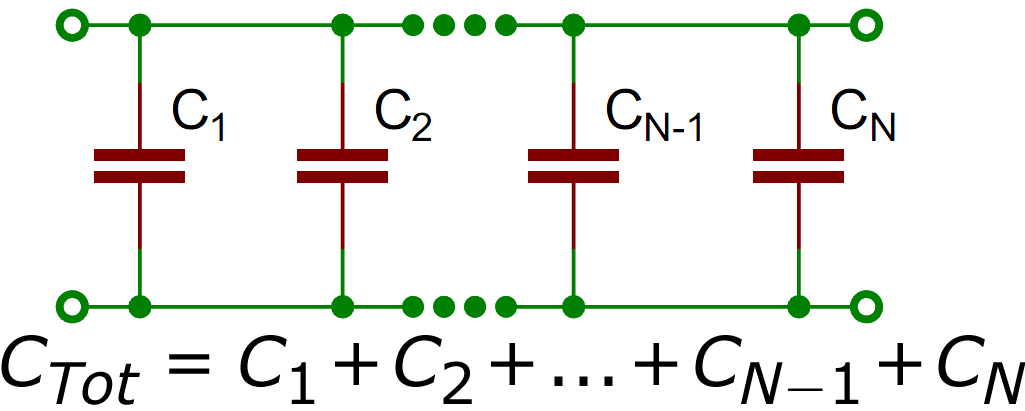
\includegraphics[width=0.8\textwidth]{./images/CapacitorsParallelConnection.png}
						\caption{Capacitors in parallel}
						\label{fig:capacitors_in_parallel}
					\end{subfigure}
					\hspace*{0.1\textwidth}
					\begin{subfigure}[h]{0.4\textwidth}
						\centering
						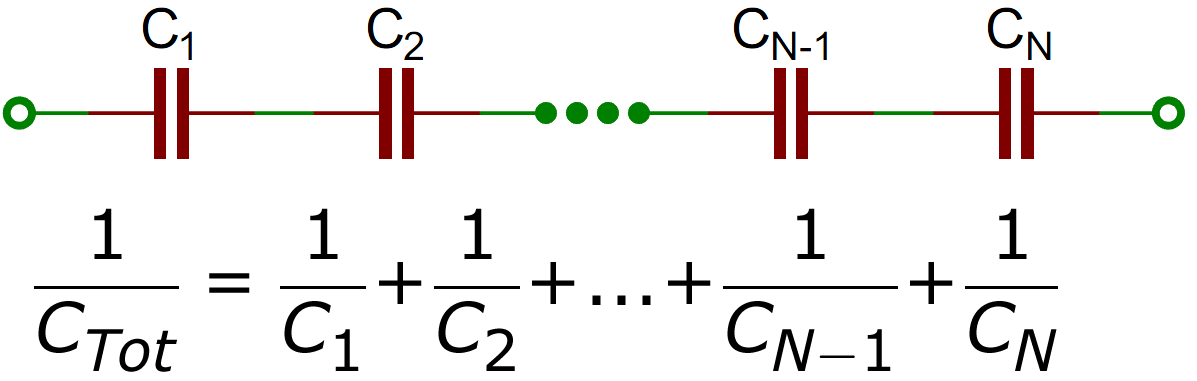
\includegraphics[width=0.8\textwidth]{./images/CapacitorsSeriesConnection.png}
						\caption{Capacitors in series}
						\label{fig:capacitors_in_series}
					\end{subfigure}

					\caption{Capacitors in series and parallel}
					\label{fig:capacitors_in_series_and_parallel}
				\end{figure}

		\subsection{Aparatus}
			\begin{itemize}
				\item 1x Breadboard
				\item 1x Power Supply
				\item 1x Multimeter
				\item 3x Resistor
				\item 1x Light Emitting Diode
				\item 2x Capacitor
				\item 2x Jumper Wires
			\end{itemize}

			\subsubsection{Breadboard}
				A breadboard is a construction base for prototyping of electronics. 
				The breadboard has strips of metal underneath the board and connect the holes on the top of the board. 
				The breadboard has two power buses, which are the red and blue lines on the side of the breadboard. 
				The red line is the positive power bus and the blue line is the negative power bus. 
				The power buses are used to supply power to the components on the breadboard.\\

				\begin{figure}[h!]
					\centering
					\begin{subfigure}{0.45\textwidth}
						\centering
						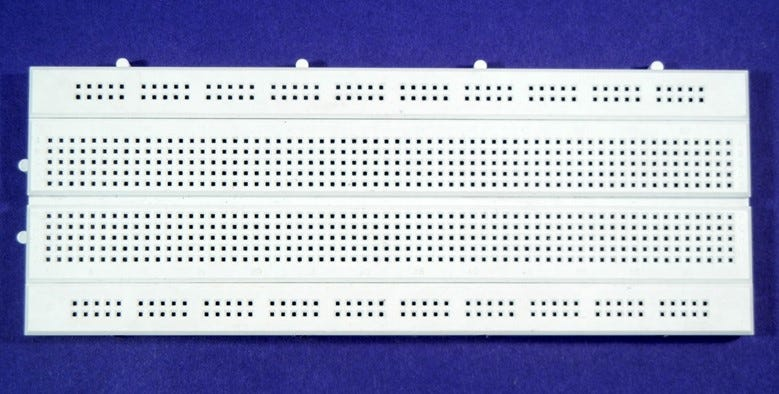
\includegraphics[width=0.8\textwidth]{./images/Breadboard.jpeg}
						\caption{Physical Breadboard}
					\end{subfigure}
					\hspace*{0.05\textwidth}
					\begin{subfigure}{0.45\textwidth}
						\centering
						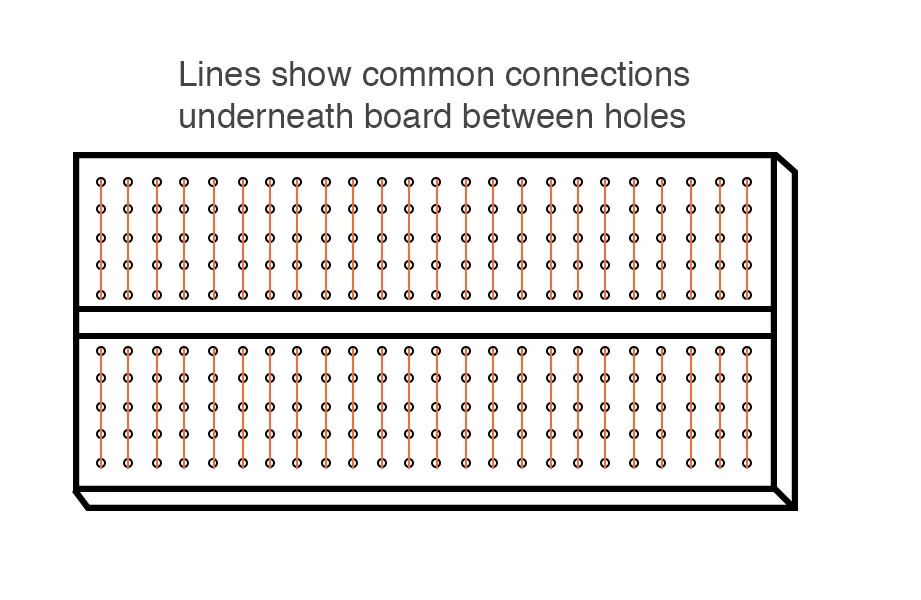
\includegraphics[width=0.8\textwidth]{./images/breadboard_diagram.png}
						\caption{Breadboard Diagram}
					\end{subfigure}
					\caption{Breadboard}
					\label{fig:breadboard}
				\end{figure}

				\pagebreak
			\subsubsection{Power Supply}
				A power supply is a device that supplies electrical energy to an electrical load. 
				The power supply has two terminals, a positive terminal, and a negative terminal. 
				The power supply is used to supply power to the circuit.\\

				\begin{figure}[h!]
					\centering
					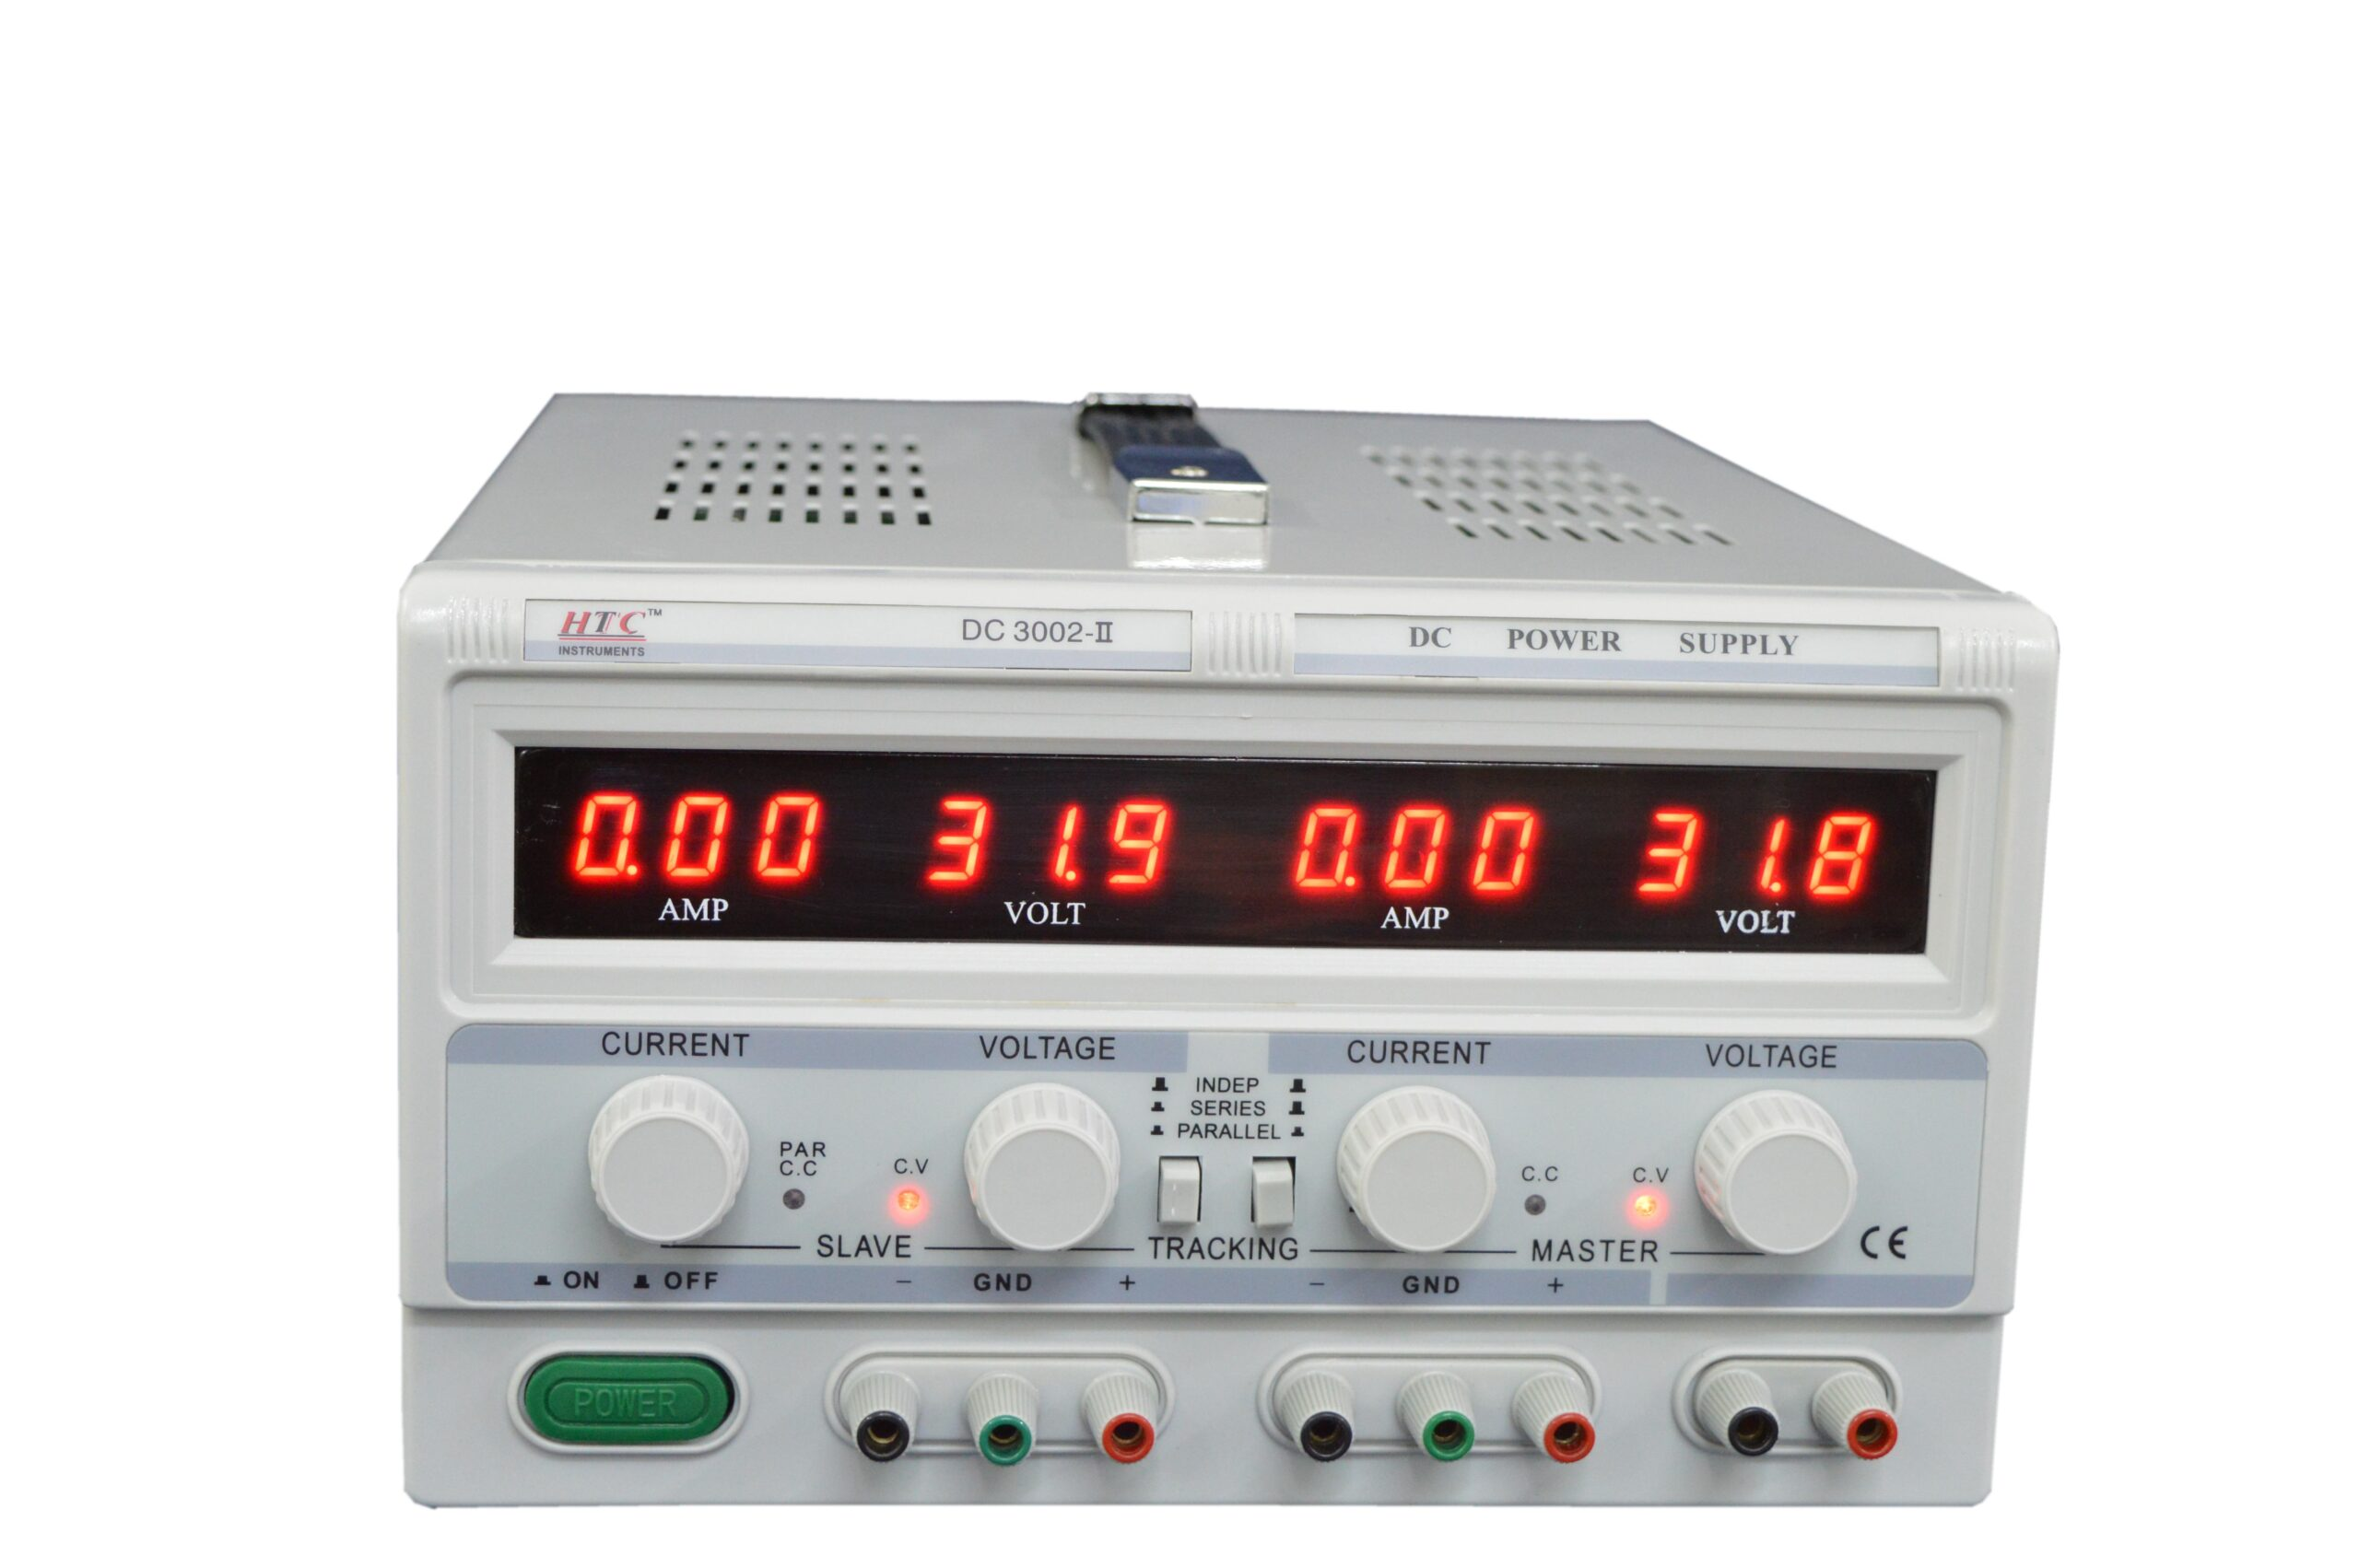
\includegraphics[width=0.5\textwidth]{./images/DC-PowerSupply.jpeg}
					\caption{Power Supply}
					\label{fig:power_supply}
				\end{figure}

			\subsubsection{Multimeter}
				A multimeter is a device that measures multiple electrical properties of the circuit. 
				In our case we will use the multimeter to measure the voltage across the capacitor, the resistance of the
				resistor, and the capacitance of our capacitors.\\

				\begin{figure}[h!]
					\centering
					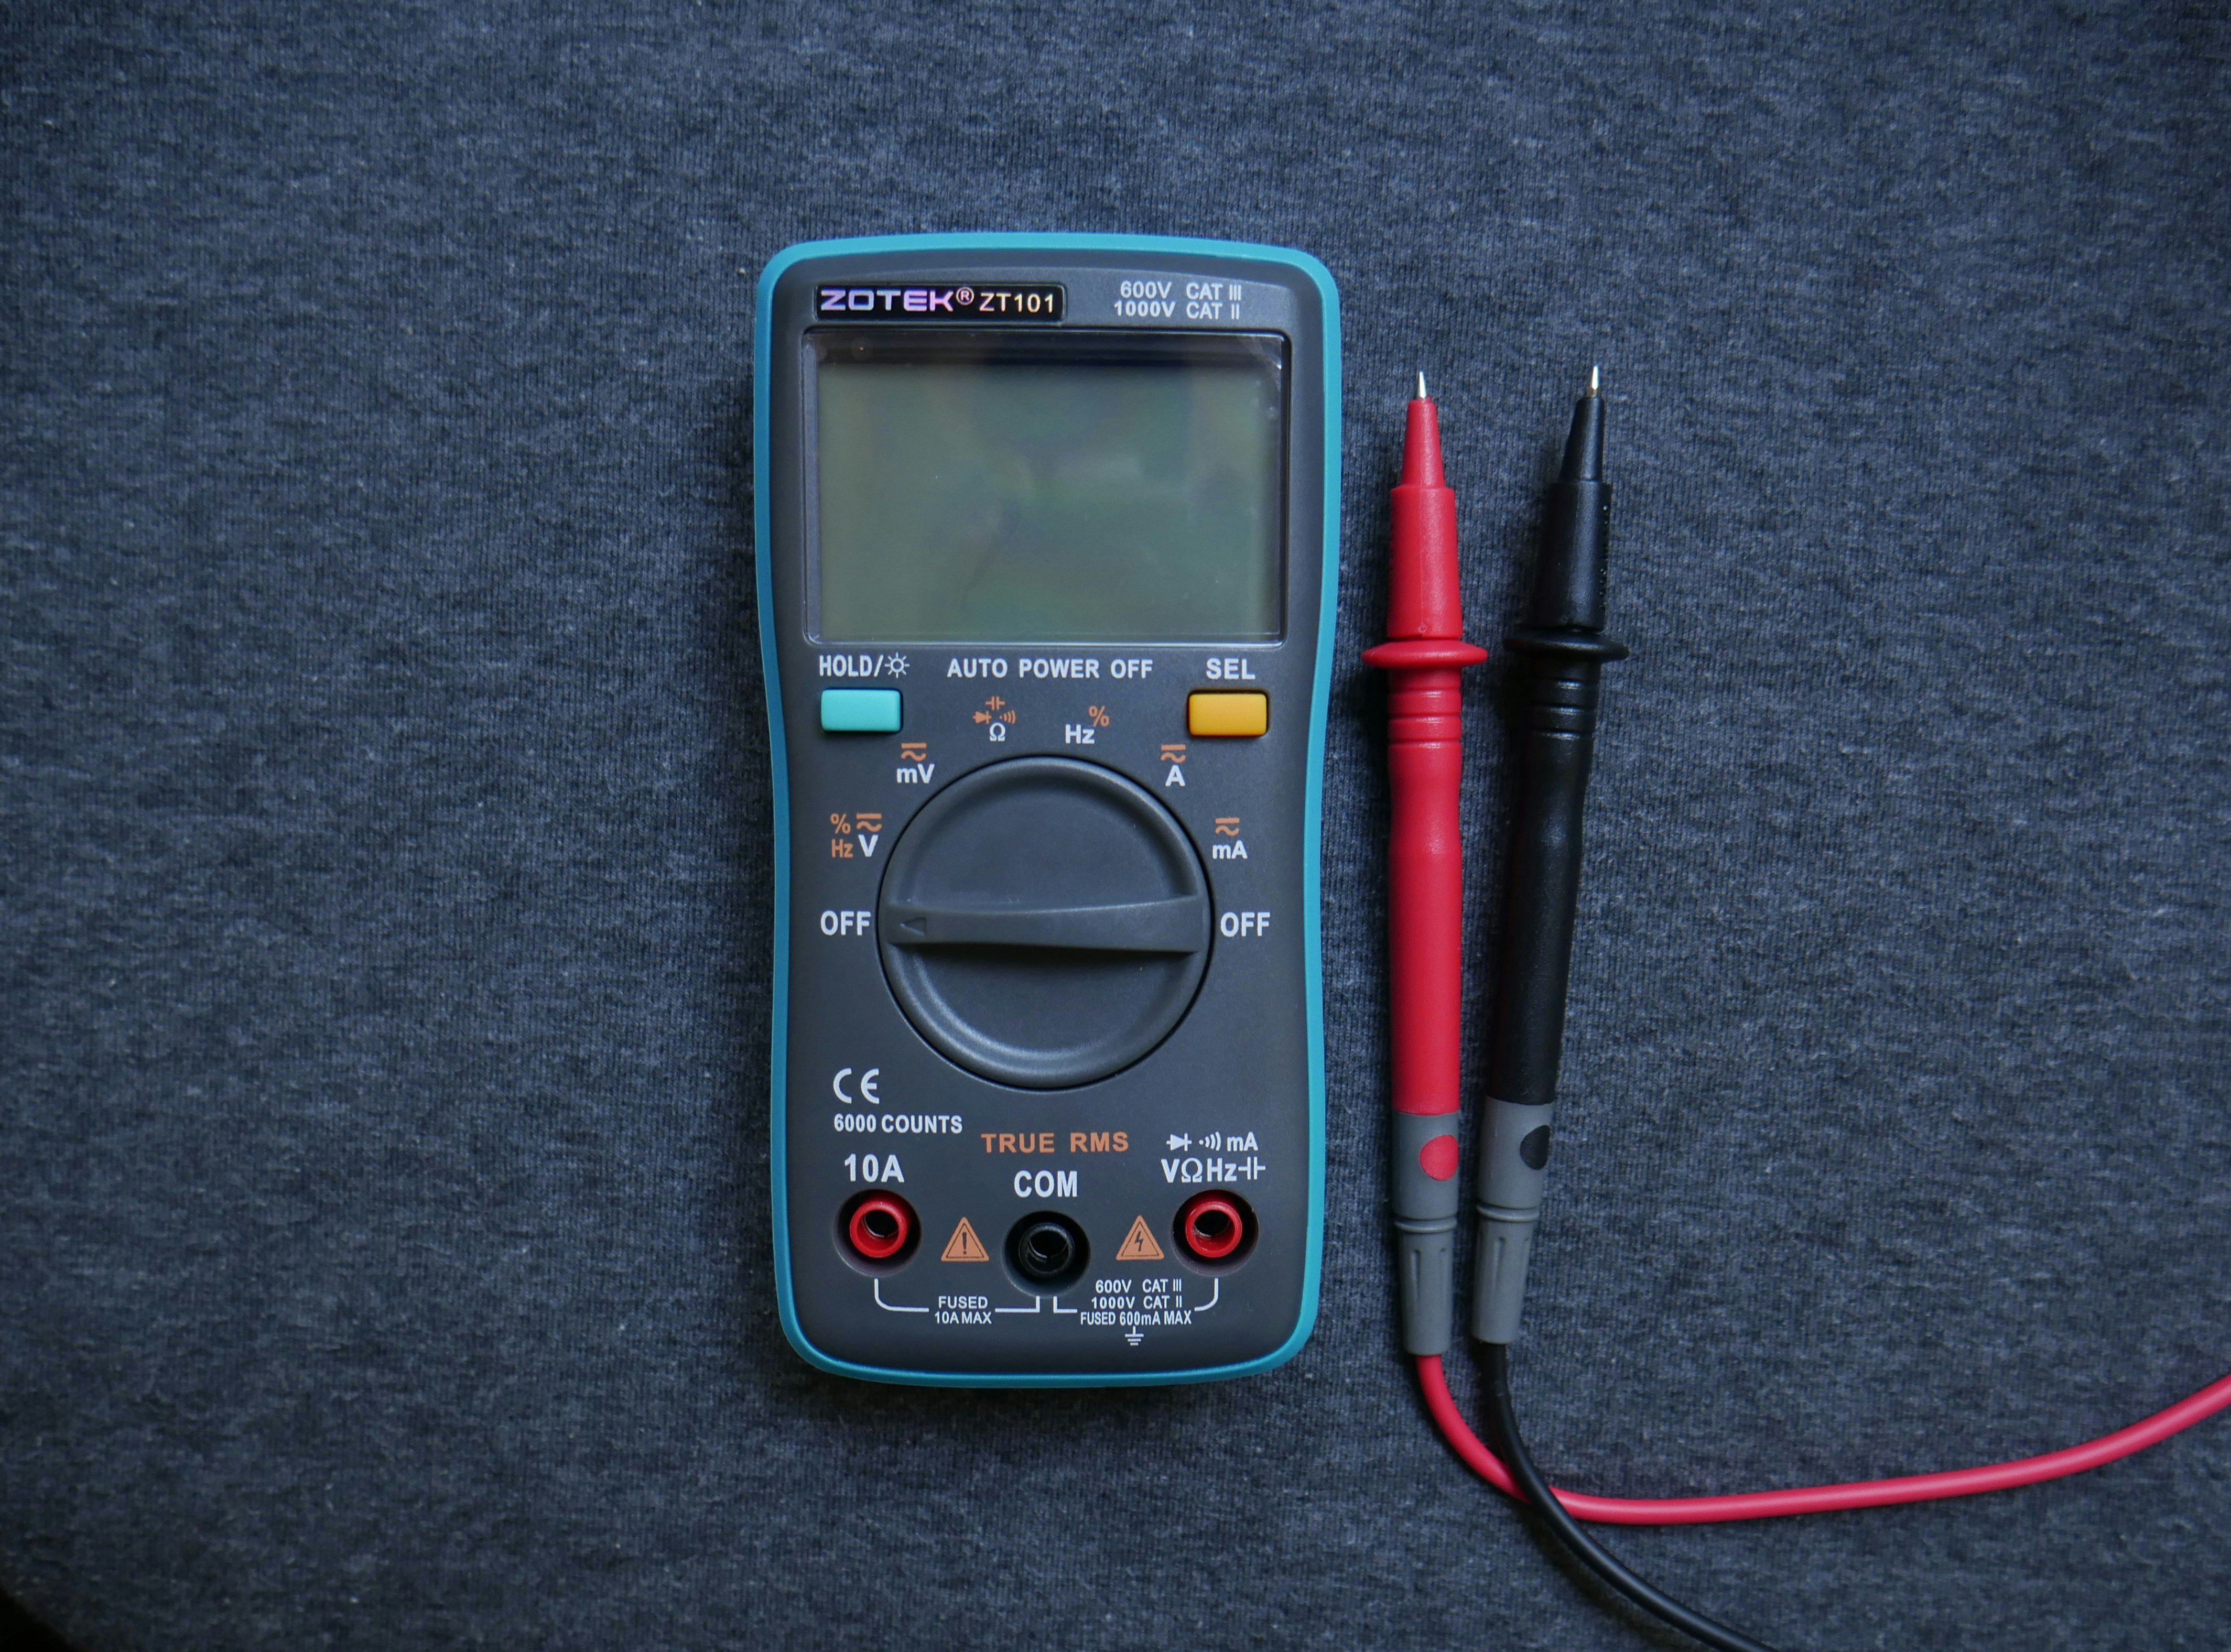
\includegraphics[width=0.5\textwidth]{./images/Multimeter.jpg}
					\caption{Multimeter}
					\label{fig:multimeter}
				\end{figure}

			\pagebreak
			\subsubsection{Resistor}
				A resistor is a passive two-terminal electrical component that implements electrical resistance as a circuit element. 
				Resistors are used to reduce current flow, divide voltages, among other uses.\\
				In this lab, we will be using three resistors: 1k$\Omega$, 10k$\Omega$, and 100k$\Omega$.\\

				\begin{figure}[h!]
					\centering
					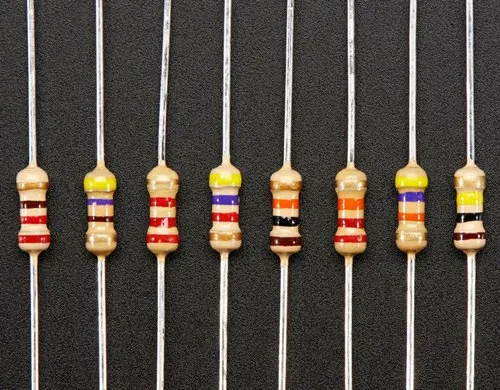
\includegraphics[width=0.4\textwidth]{./images/resistors.png}
					\caption{Resistor}
					\label{fig:resistor}
				\end{figure}

			\subsubsection{Light Emitting Diode}
				A light-emitting diode (LED) is a semiconductor light source that emits light when current flows through it. 
				LEDs are used in many applications, such as indicators, lighting, and more.\\

				\begin{figure}[h!]
					\centering
					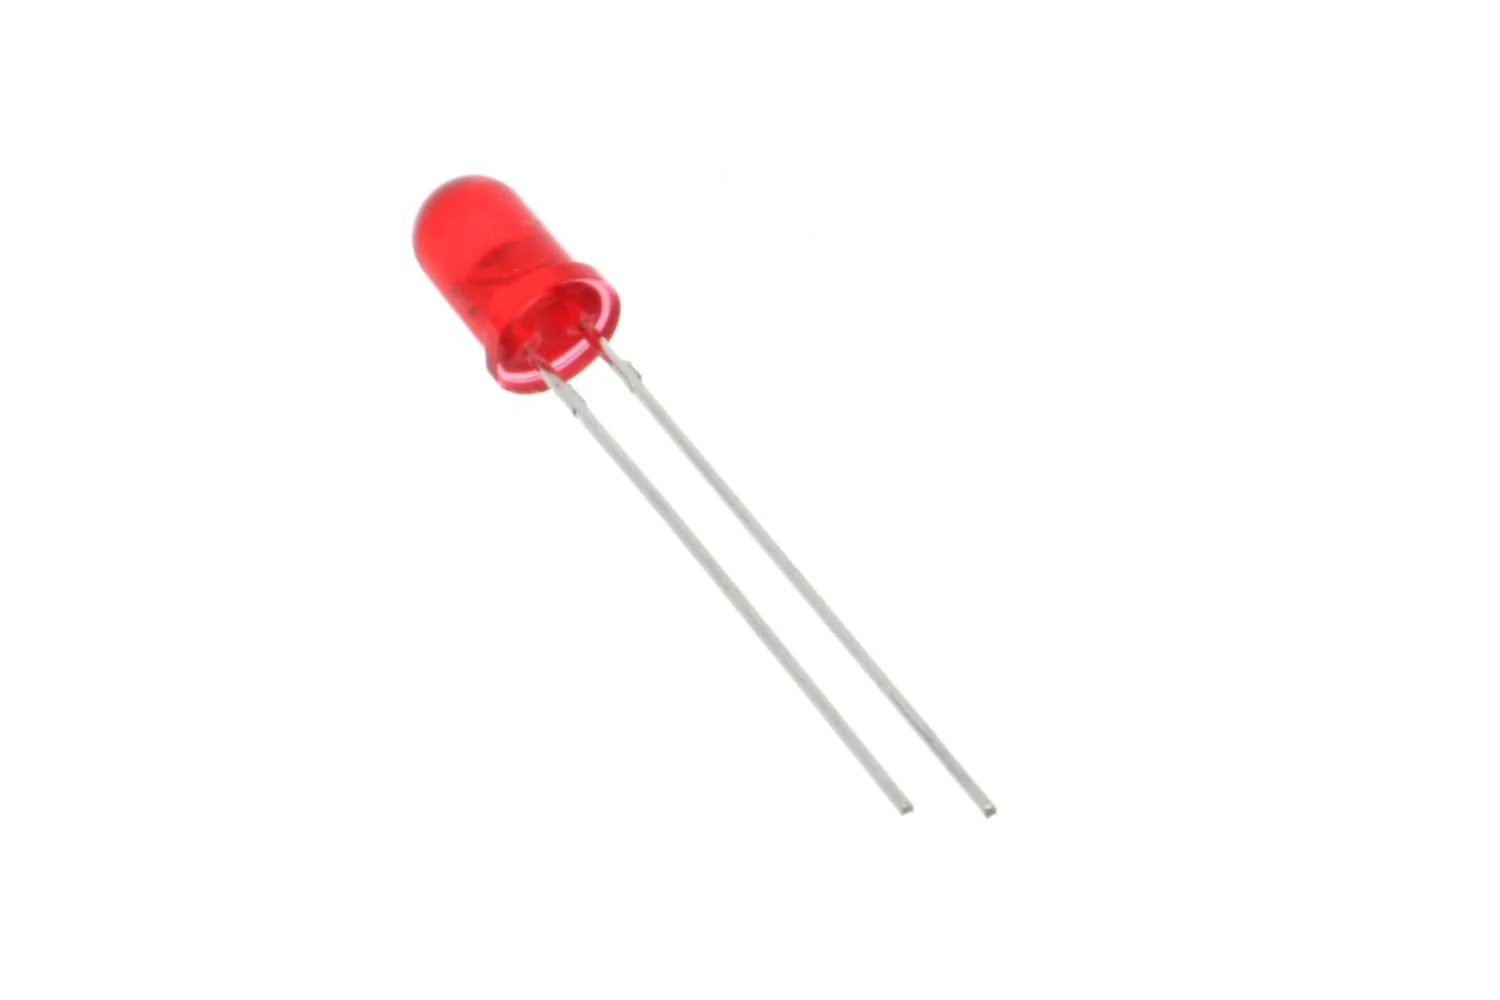
\includegraphics[width=0.4\textwidth]{./images/LED.jpeg}
					\caption{Light Emitting Diode}
					\label{fig:led}
				\end{figure}

			\subsubsection{Capacitor}
				A capacitor is a passive two-terminal electrical component that stores energy in an electric field. 
				Capacitors are used in many applications, such as filtering, timing circuits, and more.\\
				In this lab, we will be using two capacitors: 1$\mu$F.\\

				\begin{figure}[h!]
					\centering
					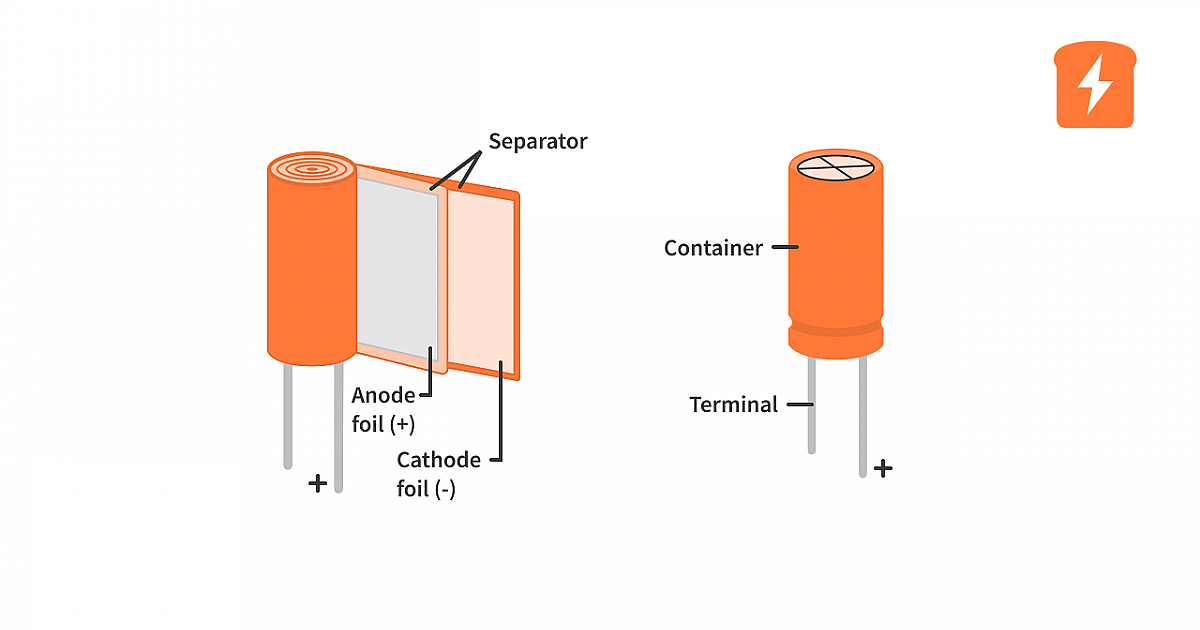
\includegraphics[width=0.4\textwidth]{./images/basics-capacitor-thumbnail.png}
					\caption{Capacitor}
					\label{fig:capacitor}
				\end{figure}

				\pagebreak
			\subsubsection{Jumper Wires}
				Jumper wires are used to connect components on the breadboard when a direct connection might be hard to make. 
				In this lab we will use jumper wires are switches.\\

				\begin{figure}[h!]
					\centering
					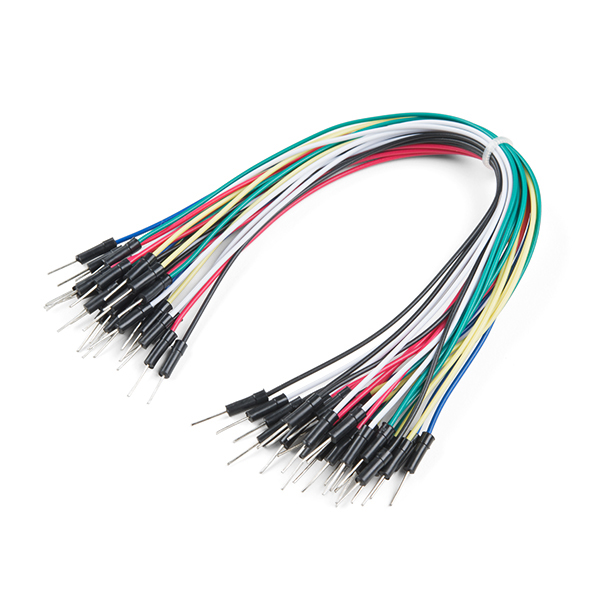
\includegraphics[width=0.4\textwidth]{./images/JumperWires.jpeg}
					\caption{Jumper Wires}
					\label{fig:jumper_wires}
				\end{figure}

				
\end{document}
